\documentclass[conference]{IEEEtran}

\usepackage{cite}
\usepackage{amsmath,amssymb,amsfonts}
\usepackage{graphicx}
\usepackage{textcomp}
\usepackage{booktabs}
\usepackage{array}
\usepackage{url}

\graphicspath{{figures/}}
\setlength{\textfloatsep}{8pt plus 2pt minus 4pt}
\setlength{\floatsep}{8pt plus 2pt minus 2pt}
\setlength{\intextsep}{8pt plus 2pt minus 2pt}

\begin{document}

\title{C.A.S.C.O.: A Smart Helmet Prototype for Fall Detection, Event Capture, and Real-Time Alerts}

\author{
\IEEEauthorblockN{Josu\'e L\'opez, \IEEEmembership{Student Member, IEEE}}
\IEEEauthorblockA{\textit{Faculty of Engineering}\\
\textit{Universidad Evang\'elica de El Salvador}\\
San Salvador, El Salvador\\
josuerlb1110@gmail.com}
\and
\IEEEauthorblockN{Jorge Larios, \IEEEmembership{Student Member, IEEE}}
\IEEEauthorblockA{\textit{Faculty of Engineering}\\
\textit{Universidad Evang\'elica de El Salvador}\\
San Salvador, El Salvador\\
romerojorge0504@gmail.com}
\and
\IEEEauthorblockN{Francisco Reyes, \IEEEmembership{Student Member, IEEE}}
\IEEEauthorblockA{\textit{Faculty of Engineering}\\
\textit{Universidad Evang\'elica de El Salvador}\\
San Salvador, El Salvador\\
Reeyes888@gmail.com}
\and
\IEEEauthorblockN{Job N. Acosta, \IEEEmembership{Member, IEEE}}
\IEEEauthorblockA{\textit{Faculty of Engineering}\\
\textit{Universidad Evang\'elica de El Salvador}\\
San Salvador, El Salvador\\
jobacosta@ieee.org}
}

\maketitle

\begin{abstract}
This paper presents C.A.S.C.O.\ (Casco Aut\'onomo con Sensores de Control y Observaci\'on), an autonomous IoT safety-helmet prototype designed to improve post-fall awareness in industrial and construction environments. The system combines an ESP32-WROOM-32, an MPU6050 inertial measurement unit, an ESP32-CAM module, and a cloud-connected software stack to detect fall events, preserve short video evidence, and notify supervisors in real time. A three-stage finite-state machine evaluates freefall, impact, and post-impact stillness using empirically selected accelerometer and gyroscope thresholds. When a fall is confirmed, the sensor node sends an ESP-NOW trigger to the camera node, which locks a seven-second pre-event JPEG buffer in PSRAM, records seven seconds after the event, uploads the resulting MJPEG clip to backend storage, and emits alerts through Socket.IO. Preliminary testing over 50 fall-like trials and 80 non-fall trials produced 92.0\% sensitivity and 92.5\% specificity. Communication tests showed 50/50 successful ESP-NOW pairing attempts with an average 5\,s pairing completion time, while the video pipeline averaged two lost frames per recorded event, 15\,s upload time, and 5\,h continuous runtime from a 5\,V, 5000\,mAh battery under repeated accident-video recording. The results support the feasibility of the low-cost architecture while showing that further classifier tuning is required before safety-critical deployment.
\end{abstract}

\begin{IEEEkeywords}
ESP-NOW, ESP32-CAM, fall detection, industrial safety, Internet of Things, MPU6050, real-time alerts, smart helmet.
\end{IEEEkeywords}

\section{Introduction}

Falls remain a major safety risk in construction work. The U.S.\ Bureau of Labor Statistics reports that, in 2024, there were 1{,}034 private-sector construction fatalities, of which 389 were falls, slips, and trips, and that 95.9\% of those events were falls to a lower level~\cite{bls2026}. OSHA's Fall Prevention Campaign likewise identifies falls as the leading cause of death in construction and cites the same BLS counts~\cite{osha2026}. NIOSH similarly identifies construction as a sector with a disproportionate share of fatal slips, trips, and falls~\cite{niosh2026}. These data motivate systems that can detect incidents quickly and help supervisors reconstruct what happened after an emergency.

C.A.S.C.O.\ addresses this need through a smart safety helmet that detects a probable fall, captures context video from before and after the event, and reports the event to web and mobile clients. The design emphasizes low-cost hardware, free-tier cloud deployment, and a simple first-use workflow: the worker powers the helmet, the camera module joins Wi-Fi once through a captive portal, and the system thereafter operates autonomously. This user-experience goal came from the project plan requirement that workers should not have to enter technical IP addresses or configure the sensor node manually.

The main contribution of this work is an end-to-end smart-helmet prototype that combines local threshold-based fall detection, ESP-NOW-based inter-device triggering, PSRAM-based pre-event video buffering, cloud event storage, and real-time web/mobile supervisor alerts. Unlike alert-only fall-detection systems, the proposed prototype preserves visual context before and after the incident while avoiding direct inbound network access to the helmet. This paper reports the implementation and integration status honestly as a prototype, not as certified safety equipment.

\section{State of the Art}

Wearable fall-detection research commonly relies on inertial sensors. Ramachandran and Karuppiah survey threshold-based and machine-learning approaches for separating falls from daily activity~\cite{ramachandran2020}. Wu \textit{et al.} report a wearable quaternion method at 97.1\% sensitivity and 98.3\% specificity versus 91.6\% and 88.7\% for an acceleration-threshold baseline on the same evaluation~\cite{wu2015}. Ruiz-Garcia \textit{et al.} present CareFall, comparing both families on public wrist IMU recordings~\cite{ruizgarcia2023}: on the Erciyes split, an SMV threshold reached 77.3\% accuracy (100\% sensitivity, 68.4\% specificity), while a random-forest model using accelerometer and gyroscope features reached 98.4\% accuracy (98.9\%, 96.7\%). Qian \textit{et al.} report a wearable IoT multilevel-threshold system with 20 volunteers at 94.88\% accuracy, 95.25\% sensitivity, and 94.5\% specificity~\cite{qian2022}.

Table~\ref{tab:sota} lists these published figures beside the C.A.S.C.O.\ baseline. They are not a head-to-head benchmark: wrist versus helmet placement, public ADL datasets versus staged student trials, and different class balances all differ. The table is included only to document a consistent literature pattern---thresholds often keep high sensitivity but lose specificity, while learning methods typically reduce false alerts when labeled data exist---which matches the failure modes in Section~\ref{sec:results}. A threshold FSM remains a justified ESP32 baseline (near 100\,Hz, no training set, interpretable states, deterministic latency). A fair on-helmet comparison with SVM, random forest, or TinyML is not claimed; it would require the same helmet IMU traces plus on-device RAM and inference-time measurements.

Campero-Jurado \textit{et al.} show that industrial helmets can host IIoT sensing and near real-time safety assessment~\cite{campero2020}. C.A.S.C.O.\ differs from many alert-only designs by adding pre/post-event video and cloud supervisor notification. Current novelty is architectural; detection-reliability claims require controlled experiments.

\begin{table*}[!t]
\centering
\caption{Published fall-detection figures versus the C.A.S.C.O.\ prototype baseline. Metrics are taken from the cited papers and are not directly comparable across sensor placements or datasets.}
\label{tab:sota}
{\scriptsize
\begin{tabular}{@{}l l l l c c c@{}}
\toprule
\textbf{Work} & \textbf{Sensing} & \textbf{Approach} & \textbf{Evaluation} & \textbf{Sens.} & \textbf{Spec.} & \textbf{Acc.} \\
\midrule
Wu \textit{et al.}~\cite{wu2015} & wearable IMU & quaternion method & published lab study & 97.1\% & 98.3\% & -- \\
Wu \textit{et al.}~\cite{wu2015} & wearable IMU & accel.\ threshold & same study & 91.6\% & 88.7\% & -- \\
CareFall~\cite{ruizgarcia2023} & wrist IMU & SMV threshold & Erciyes (public) & 100\% & 68.4\% & 77.3\% \\
CareFall~\cite{ruizgarcia2023} & wrist IMU & RF, acc.+gyr. & Erciyes (public) & 98.9\% & 96.7\% & 98.4\% \\
Qian \textit{et al.}~\cite{qian2022} & wearable IMU & multilevel threshold & 20 volunteers & 95.25\% & 94.5\% & 94.88\% \\
C.A.S.C.O.\ (this work) & helmet IMU & 3-stage FSM & 3 students, 130 staged trials & 92.0\% & 92.5\% & 92.3\% \\
\bottomrule
\end{tabular}
}
\end{table*}

\section{System Architecture}

The C.A.S.C.O.\ prototype is divided into four main layers: an inertial sensing node, an edge camera node, a backend and storage layer, and web/mobile user interfaces. Fig.~\ref{fig:architecture} shows the end-to-end architecture. The sensor node is based on an ESP32-WROOM-32 connected to an MPU6050 over I2C. It samples acceleration and angular velocity at approximately 100\,Hz and runs the fall-detection finite-state machine. When a fall is confirmed, it sends a compact trigger message to the ESP32-CAM using ESP-NOW.

\begin{figure}[!t]
\centering
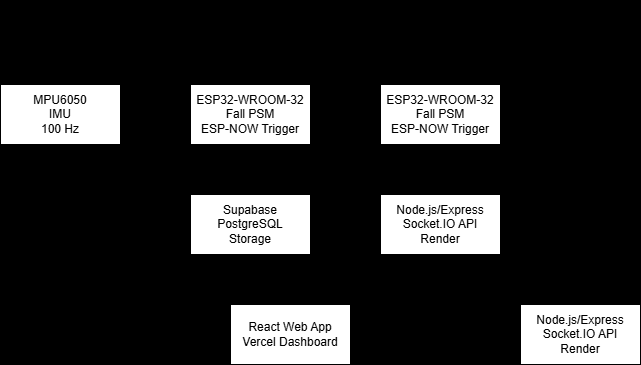
\includegraphics[width=0.92\columnwidth]{fig1_architecture.png}
\caption{C.A.S.C.O.\ system architecture.}
\label{fig:architecture}
\end{figure}

The ESP32-CAM is responsible for image capture, event recording, upload, and streaming. During normal operation it maintains a circular buffer of JPEG frames in PSRAM. At the time of a fall trigger, it preserves the last seven seconds of pre-event imagery and captures seven seconds of post-event frames. It then exports the event as an MJPEG clip, uploads it through HTTPS, and sends a backend event notification. The backend runs on Node.js/Express with Socket.IO for real-time communication, PostgreSQL for event/device data, and Supabase Storage for clips and snapshots.

\section{Embedded Hardware and Communication Design}

\subsection{Sensor Node}
The sensor node uses an ESP32-WROOM-32 and an MPU6050 inertial measurement unit. The MPU6050 integrates a 3-axis accelerometer and a 3-axis gyroscope in a single 6-axis motion device~\cite{tdk2013}. In the current prototype, the accelerometer is configured for $\pm2g$, the gyroscope for $\pm250~\mathrm{deg/s}$, and the digital low-pass filter for 20\,Hz. The sampling loop uses an approximate 10\,ms delay, producing an effective rate near 100\,Hz.

The fall detector computes acceleration magnitude and gyroscope magnitude from the raw sensor values. It does not depend on Wi-Fi credentials or a router IP address. The only nonvolatile peer information stored by the sensor node is the ESP32-CAM MAC address obtained during ESP-NOW pairing. This keeps the WROOM firmware focused on deterministic local sensing and avoids user-facing configuration complexity.

\subsection{Camera Node}
The camera node uses an AI-Thinker ESP32-CAM with an OV2640 camera, 4\,MB PSRAM, and 4\,MB flash. The camera is configured for QVGA resolution at $320\times240$ pixels, JPEG quality 12, and two frame buffers. PSRAM holds the circular pre-event buffer and the combined pre/post-event frame set during event capture.

The ESP32-CAM also manages Wi-Fi setup. On first use it launches a captive portal named CASCO-Setup using WiFiManager and displays the device identifier. After joining the user network, it generates a CASCO-XXXXXX identifier from the MAC suffix, auto-registers with the backend, and stores the returned device API token in nonvolatile storage. This design centralizes Wi-Fi and Internet communication in the camera node while leaving the WROOM node independent from network setup.

\subsection{ESP-NOW Pairing and Triggering}
ESP-NOW was selected for communication between the sensor and camera nodes. Espressif defines ESP-NOW as a connectionless Wi-Fi communication protocol in which application data is transmitted directly between devices without a conventional Wi-Fi connection, and notes that it can operate device-to-device without a router forwarding packets~\cite{espressifespnow}. These properties suit a helmet architecture in which the sensor node should not depend on router association or an IP address.

The pairing flow uses a broadcast byte and an acknowledgment byte. The camera node broadcasts 0xAA on the configured channel until the WROOM node receives it, stores the sender MAC address, registers it as a peer, and replies with 0xBB. On later restarts, the WROOM loads the stored camera MAC address and sends 0xBB again to restore the paired state. A confirmed fall is transmitted as a compact FallMessage containing a boolean fall flag and a floating-point severity value.

A key engineering correction was moving expensive operations out of the ESP-NOW receive callback. The callback runs in a Wi-Fi task context; performing HTTP requests or heavy PSRAM work inside the callback caused instability. The corrected design only updates volatile flags inside the callback, while the main loop performs event capture and backend communication.

\section{Fall Detection Algorithm}

The fall-detection algorithm is a three-stage finite-state machine, shown in Fig.~\ref{fig:fsm}. The machine transitions from IDLE to FREEFALL\_DETECTED when acceleration magnitude drops below 0.5\,g. If an impact greater than 2.5\,g occurs within the configured time window and the gyroscope magnitude changes sharply, the state advances to IMPACT\_DETECTED. The algorithm then requires approximately 1.5\,s of post-impact stillness before confirming the fall and sending the alert.

\begin{figure}[!t]
\centering
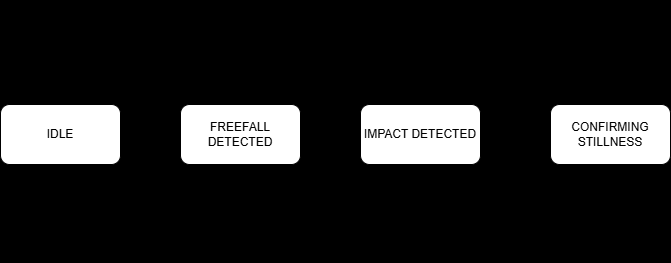
\includegraphics[width=0.92\columnwidth]{fig2_fsm.png}
\caption{Three-stage fall-detection finite-state machine.}
\label{fig:fsm}
\end{figure}

The firmware uses the current acceleration magnitude, $|a|$, and the current and previous gyroscope magnitudes to estimate whether the motion sequence is consistent with a fall. The severity value transmitted to the camera node is the measured impact acceleration divided by the 2.5\,g impact threshold. This ratio allows later backend versions to treat stronger impacts differently without increasing the ESP-NOW message size.

This threshold-based method was chosen for transparency and ease of calibration. The thresholds were selected empirically during prototype development by observing the intended freefall-impact-stillness sequence and reducing immediate false triggers from ordinary handling. The method remains a prototype baseline rather than certified safety equipment; Section~\ref{sec:results} shows that additional threshold tuning or learning-based classification is needed to reduce missed fall events.

\section{Video Buffering and Cloud Alert Pipeline}

The ESP32-CAM maintains a 70-frame circular JPEG buffer at 10\,FPS, representing seven seconds of pre-event video. On a fall trigger, the firmware locks and copies this pre-buffer, then records an additional 70 post-event frames. The total event clip therefore contains 140 frames, approximately 14\,s of incident context. The prototype estimates about 1.4\,MB of PSRAM use per full event frame set. Events are stored as MJPEG rather than H.264 because the ESP32-CAM captures JPEG frames and does not provide hardware H.264 encoding.

In addition to event clips, the camera node supports two forms of live viewing. A local MJPEG stream is available on the same network through the \texttt{/stream} route, while remote viewing is implemented as a pseudo-stream: the camera posts raw JPEG frames to the backend at 5\,FPS, and the backend relays them to joined clients via Socket.IO. This avoids direct inbound connections to the helmet and works behind common network address translation.

The backend uses Node.js and Express routes for authentication, device management, event creation, file uploads, snapshots, and frame streaming. User clients authenticate with JWTs, while devices authenticate with API tokens. PostgreSQL tables store users, devices, and events. Socket.IO rooms isolate real-time traffic by device identifier~\cite{socketio2026}. Supabase Storage holds event clips and snapshots; the product documentation distinguishes public and private buckets and signed URLs for time-limited access~\cite{supabase2026}.

Two client interfaces were implemented. The React web dashboard provides login, registration, device linking, device deletion, live frames, and an event list. The Flutter Android app mirrors the same core workflow, stores the JWT locally, connects to Socket.IO, and displays frame updates using \texttt{Image.memory} with gapless playback to reduce flicker.

\section{Experimental Methodology}

A controlled prototype validation was conducted to address detection reliability, false alerts, communication behavior, video stability, upload delay, and runtime. The evaluation separated fall-like events from non-fall activities so that true positives, false negatives, true negatives, and false positives could be reported separately.

Tests were performed with the helmet worn by a person on a floor surface, using both indoor and outdoor settings. No result pattern was attributed to the test location, and the present dataset is \emph{not} split into indoor versus outdoor counts because that breakdown was not recorded as a separate experimental factor. Three university-student participants with little height variation performed the trials. No occupational construction workers were enrolled, and the falls were simulated (not accidental) on a floor surface. Ground truth was assigned manually for each trial before the firmware output was compared with the expected fall or non-fall label. The 92.0\% / 92.5\% figures reported below are therefore a prototype baseline on a small, demographically narrow, staged-motion cohort; they are not a generalizable industrial result.

The fall-like set contained 50 trials: 20 forward-fall trials, 10 lateral-fall trials, 15 backward-fall trials, and 5 helmet drop/impact simulations. The non-fall set contained 80 trials representing ordinary helmet and worker motions; the observed false alerts were associated mainly with sudden strong movements and rough helmet placing or dropping. Communication performance was evaluated with 50 ESP-NOW pairing attempts, and the video and power tests measured frame loss, stream interruption during recording, upload time, and continuous runtime. The tests should be interpreted as validation of the implemented prototype thresholds, not as final field validation or certification evidence.

The primary classifier metrics were sensitivity $\mathrm{TP}/(\mathrm{TP}+\mathrm{FN})$, specificity $\mathrm{TN}/(\mathrm{TN}+\mathrm{FP})$, false-alert rate $\mathrm{FP}/(\mathrm{FP}+\mathrm{TN})$, accuracy $(\mathrm{TP}+\mathrm{TN})/N$, precision $\mathrm{TP}/(\mathrm{TP}+\mathrm{FP})$, and F1-score. ESP-NOW timing was reported as pairing completion time; fall-trigger delivery latency after pairing was not isolated as a separate measurement.

\begin{table}[!t]
\centering
\caption{Prototype Configuration Parameters}
\label{tab:config}
\begin{tabular}{@{}ll@{}}
\toprule
\textbf{Parameter} & \textbf{Value} \\
\midrule
IMU sampling rate & approx.\ 100 Hz \\
Fall sequence & freefall, impact, stillness \\
Pre-event buffer & 7\,s, 70 JPEG frames \\
Post-event recording & 7\,s, 70 JPEG frames \\
Total clip length & approx.\ 14\,s, 140 frames \\
Remote stream rate & 5 FPS \\
Camera resolution & QVGA, $320\times240$ \\
ESP-NOW channel & 11, configurable \\
Backend deployment & Render free-tier service \\
Storage/database & Supabase Storage and PostgreSQL \\
\bottomrule
\end{tabular}
\end{table}

\section{Results and Discussion}
\label{sec:results}

The implemented prototype currently supports fall detection, automatic ESP-NOW pairing, automatic device registration, Wi-Fi configuration through a captive portal, PSRAM-based pre/post-event capture, clip upload, real-time Socket.IO alerts, remote frame streaming at 5\,FPS, a deployed web dashboard, and a Flutter Android application. Table~\ref{tab:config} summarizes the configuration parameters, Table~\ref{tab:validation} reports the fall-scenario and classifier results, and Table~\ref{tab:systemperf} summarizes communication, video, upload, and power measurements.

\begin{figure}[!t]
\centering
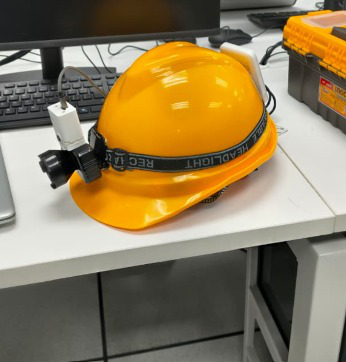
\includegraphics[width=0.58\columnwidth]{fig3_prototype.png}
\caption{Physical C.A.S.C.O.\ smart-helmet prototype used during controlled fall-like and non-fall validation trials.}
\label{fig:prototype}
\end{figure}

\begin{table}[!t]
\centering
\caption{Controlled Validation and Fall-Scenario Results}
\label{tab:validation}
{\footnotesize
\begin{tabular}{@{}p{0.21\columnwidth} c p{0.26\columnwidth} p{0.30\columnwidth}@{}}
\toprule
\textbf{Scenario} & \textbf{Trials} & \textbf{Result counts} & \textbf{Primary metric} \\
\midrule
Forward fall & 20 & TP=19, FN=1 & Sensitivity 95.0\% \\
Side/lateral fall & 10 & TP=9, FN=1 & Sensitivity 90.0\% \\
Backward fall & 15 & TP=14, FN=1 & Sensitivity 93.3\% \\
Helmet drop/impact & 5 & TP=4, FN=1 & Sensitivity 80.0\% \\
Fall-like total & 50 & TP=46, FN=4 & Sensitivity 92.0\%; avg latency 2\,s \\
Non-fall activities & 80 & TN=74, FP=6 & Specificity 92.5\%; false-alert rate 7.5\% \\
Combined classifier & 130 & Correct=120, errors=10 & Accuracy 92.3\%; precision 88.5\%; F1 90.2\% \\
\bottomrule
\end{tabular}
}
\end{table}

\begin{table}[!t]
\centering
\caption{System Performance Measurements}
\label{tab:systemperf}
{\footnotesize
\begin{tabular}{@{}p{0.17\columnwidth} p{0.35\columnwidth} p{0.35\columnwidth}@{}}
\toprule
\textbf{Subsystem} & \textbf{Test scope} & \textbf{Measured result} \\
\midrule
ESP-NOW & 50 pairing attempts & 50/50 successful; avg pairing completion time 5\,s \\
Recorded video & Event recording under accident-video load & Avg 2 frames lost per recorded clip \\
Remote stream & Live pseudo-stream while recording & Avg 2\,s video loss during event recording \\
Upload pipeline & 14\,s MJPEG event clip & Avg upload time 15\,s \\
Power & 5\,V, 5000\,mAh battery under repeated accident-video recording & 5\,h measured runtime; theoretical heavy-load estimate 5--6.25\,h \\
\bottomrule
\end{tabular}
}
\end{table}

Table~\ref{tab:validation} already reports the 46/4 and 74/6 counts (92.0\% sensitivity, 92.5\% specificity, 92.3\% accuracy). False negatives occurred when post-impact stillness was not reached after an otherwise plausible freefall-impact sequence; false positives were mainly sudden handling and rough helmet placement. Pairing time (5\,s) is setup time, not post-pair trigger latency. Upload (15\,s) is clip availability, not first-alert latency, which was not isolated. The 5\,V, 5000\,mAh pack is nominally about $25~\mathrm{Wh}$; at roughly 0.8--1.0\,A under recording/upload/stream load the calculated range is 5--6.25\,h, consistent with the 5\,h stress-test measurement.

\subsection{Environmental robustness (preliminary)}
IMU thresholds do not encode indoor versus outdoor location, and the documented detection failures are motion-pattern failures (stillness not reached; abrupt handling) rather than a location effect. Indoor and outdoor trials were performed, but no per-environment metric table exists, so robustness remains an open experimental item. Engineering limits that were not quantified here include tool vibration, rain, RF congestion, metal-structure shielding, ladder work, helmet heat, and camera degradation from dust, glare, or low light. QVGA JPEG at 10\,FPS (buffer) and 5\,FPS (remote stream) would still fire a detection if the IMU sequence matches, but evidence quality would drop. ESP-NOW requires a shared channel; site Wi-Fi congestion and metal structures can affect pairing, triggering, and the observed 15\,s HTTPS upload. The 5\,h runtime is a heavy-load bound under repeated recording; idle patrol time would be longer, but thermal and vibration behavior on a worn helmet were not measured.

\section{Deployment, Scalability, Privacy, and Cybersecurity}

First-use setup is a camera-node captive portal; charging hardware is not in the prototype. Render/Supabase free tiers are suitable for development, not an industrial SLA. A 7.5\% false-alert rate on non-fall trials would be unacceptable on a large crew. Each helmet is one camera plus one Socket.IO room, so $N$ workers imply $N$ Wi-Fi clients and about 1.4\,MB MJPEG per stored event, plus free-tier CPU/bandwidth limits. ESP-NOW here is pairwise (sensor--camera), not a site mesh.

Recording is event-triggered, not continuous; public clip URLs exist only for development. Production use requires private buckets, signed URLs, role-based access, retention limits, and documented worker consent~\cite{supabase2026}. The backend already separates user JWTs from device tokens and uses HTTPS. Unresolved prototype gaps: ESP-NOW LMK/CCMP is not described as enabled; tokens are not rotated on a schedule; clip access is not audited; the helmet is an unattended IoT endpoint; Socket.IO room membership is the live-frame authorization boundary~\cite{socketio2026}.

\section{Engineering Challenges and Design Decisions}

Implementation issues that shaped the architecture include ESP-NOW channel alignment between the WROOM and camera nodes, \texttt{WiFiClientSecure} handling for HTTPS from the camera, registering \texttt{/stream/frame} before JSON body parsing so raw JPEG bodies were not consumed by middleware, and generating the device identifier after Wi-Fi initialization to avoid a zeroed MAC-derived identifier. Design tradeoffs were explicit: ESP-NOW replaced local HTTP to avoid IP discovery; PSRAM buffering replaced SD-card dependence; WebSocket relaying replaced direct camera streaming for NAT traversal; and free-tier infrastructure kept development deployment cost at zero.

\section{Limitations and Future Work}

The current prototype has important limitations. The fall detector missed 4 of 50 fall-like events (8.0\% miss rate) and generated 6 false alerts in 80 non-fall trials (7.5\% false-alert rate). Those rates are a quantitative prototype baseline on three similar-height students performing staged motions; they do not demonstrate reliability for safety-critical or occupational deployment. The false-negative observations suggest that the stillness stage should be retuned or complemented by additional features, while the false positives indicate that abrupt handling and rough helmet placement need stronger rejection logic. The event clip format is MJPEG rather than a compressed inter-frame codec, remote streaming still loses about two seconds during event recording, and public clip URLs are not suitable for sensitive industrial video.

A future detection study should enroll a larger occupational cohort (a target of at least 15 workers across trades), mixed height, weight, and age, and both sexes, and should report per-participant as well as pooled sensitivity and specificity so that overfitting to one body type is visible. Motions should include crouching, climbing, jumping, helmet donning/doffing, hammering, and repeated impacts. A future robustness study should treat environment as a factor (surface, lighting, RF load, tool vibration) rather than pooling indoor/outdoor trials. A future algorithm comparison should log helmet IMU windows and evaluate a learning-based classifier against the frozen threshold machine on the same traces, including on-device memory and latency, rather than borrowing wrist-dataset scores from the literature. Other engineering follow-ups include charging electronics, Firebase Cloud Messaging, binary streaming, private storage with signed URLs, iOS support, and OTA firmware updates.

\section{Conclusion}

C.A.S.C.O.\ is a low-cost smart-helmet prototype that combines ESP32 sensing, ESP-NOW, PSRAM video buffering, cloud storage, and Socket.IO alerts. On the staged 130-trial set it reached 92.0\% sensitivity and 92.5\% specificity, with 50/50 pairing, 15\,s average upload, and 5\,h runtime under repeated recording. These figures are a prototype baseline, not a field-safety result. Missed detections, stream gaps during recording, privacy controls, cohort diversity, and environment-factor tests remain open.

\section*{Acknowledgment}
The authors acknowledge Eng.\ Job Acosta, instructor of Embedded Systems and Hardware Description Language at the Universidad Evang\'elica de El Salvador, Faculty of Engineering, for academic guidance. The authors also thank Jorge Romero and Francisco Reyes, students who participated in prototype testing.

\begin{thebibliography}{12}

\bibitem{bls2026}
U.S.\ Bureau of Labor Statistics, ``National Safety Stand-Down highlights fall hazards in construction,'' \textit{The Economics Daily}, Aug.\ 18, 2026. [Online]. Available: \url{https://www.bls.gov/opub/ted/2026/national-safety-stand-down-highlights-fall-hazards-in-construction.htm}

\bibitem{osha2026}
Occupational Safety and Health Administration, ``OSHA's Fall Prevention Campaign,'' U.S.\ Department of Labor. [Online]. Available: \url{https://www.osha.gov/stop-falls}

\bibitem{niosh2026}
C.\ Socias-Morales, J.\ Bunting, R.\ Greenberg, and E.\ J.\ Haas, ``Construction Falls: Progress and Prevention,'' National Institute for Occupational Safety and Health, Apr.\ 20, 2026. [Online]. Available: \url{https://www.cdc.gov/niosh/bulletin/2026/falls-stand-down-2026.html}

\bibitem{ramachandran2020}
A.\ Ramachandran and A.\ Karuppiah, ``A Survey on Recent Advances in Wearable Fall Detection Systems,'' \textit{BioMed Research International}, vol.\ 2020, Art.\ no.\ 2167160, 2020, doi: 10.1155/2020/2167160.

\bibitem{wu2015}
F.\ Wu, H.\ Zhao, Y.\ Zhao, and H.\ Zhong, ``Development of a Wearable-Sensor-Based Fall Detection System,'' \textit{International Journal of Telemedicine and Applications}, vol.\ 2015, Art.\ no.\ 576364, 2015, doi: 10.1155/2015/576364.

\bibitem{ruizgarcia2023}
J.\ C.\ Ruiz-Garcia, R.\ Tolosana, R.\ Vera-Rodriguez, and C.\ Moro, ``CareFall: Automatic Fall Detection through Wearable Devices and AI Methods,'' in \textit{Proc.\ Workshop on Advances of Mobile and Wearable Biometrics (WAMWB 2023)}, CEUR Workshop Proc., vol.\ 3517, pp.\ 51--57, 2023. [Online]. Available: \url{https://ceur-ws.org/Vol-3517/paper4.pdf}

\bibitem{qian2022}
Z.\ Qian \textit{et al.}, ``Development of a Real-Time Wearable Fall Detection System in the Context of Internet of Things,'' \textit{IEEE Internet of Things Journal}, vol.\ 9, no.\ 21, pp.\ 21999--22007, Nov.\ 2022, doi: 10.1109/JIOT.2022.3181701.

\bibitem{campero2020}
I.\ Campero-Jurado, S.\ M\'arquez-S\'anchez, J.\ Quintanar-G\'omez, S.\ Rodr\'iguez, J.\ M.\ Corchado, and J.\ M.\ Molina, ``Smart Helmet 5.0 for Industrial Internet of Things Using Artificial Intelligence,'' \textit{Sensors}, vol.\ 20, no.\ 21, Art.\ no.\ 6241, 2020, doi: 10.3390/s20216241.

\bibitem{tdk2013}
TDK InvenSense, ``MPU-6000 and MPU-6050 Product Specification, Revision 3.4,'' Aug.\ 19, 2013. [Online]. Available: \url{https://invensense.tdk.com/wp-content/uploads/2015/02/MPU-6000-Datasheet1.pdf}

\bibitem{espressifespnow}
Espressif Systems, ``ESP-NOW,'' \textit{ESP-IDF Programming Guide}, v5.4. [Online]. Available: \url{https://docs.espressif.com/projects/esp-idf/en/v5.4/esp32/api-reference/network/esp_now.html}

\bibitem{socketio2026}
Socket.IO, ``Server API,'' Socket.IO Documentation, v4. [Online]. Available: \url{https://socket.io/docs/v4/server-api/}

\bibitem{supabase2026}
Supabase, ``Storage,'' Supabase Documentation. [Online]. Available: \url{https://supabase.com/docs/guides/storage}

\end{thebibliography}

\end{document}
